\documentclass[a4paper,10pt]{article}
\usepackage{amsmath}
\usepackage{amstext}
\usepackage{amsbsy}
\usepackage{graphicx}
\usepackage{fancyvrb}
%\usepackage{algorithm}
%\usepackage{algorithmic}

\title{ Las Vegas Geometry }

\author{Eray {\"O}zkural}

\date{\today}

\begin{document}

\maketitle

\section{Introduction}

This project is concerned with implementation of a general purpose
randomized scheme for a variety of geometric algorithms. The work
draws from recent results regarding properties of random subsets of
geometric objects. In the paper I have been studying the authors
propose a number of new non-deterministic algorithms, some of which
have better bounds than previously known algorithms. The interesting
aspect of the algorithms is that they share a general structure, and
their expected running times arise from sharp bounds of this general
structure.

Among these algorithms is an $O(A + nlogn)$ algorithm to find all
intersecting pairs of a set of line segments and another algorithm
computes the convex hull of a set of points in $O(nlogn)$ for $d=3$
and $O(n^ {\lfloor d/2 \rfloor})$ for $d>3$. \footnote{All time bounds
  are expected time} The diameter of a set of points in $E^3$ is
computed in $O(nlogn)$ time and also included is an algorithm for
half-space range reporting. The paper has in addition theoretical
results such as tight bounds for $(\leq k)$-sets and proofs for higher
order Voronoi diagrams.

As such, the paper in fact condenses a large number of results in a
technical exposition and it is impossible to test all the ideas because of
its breadth. Many problems are tackled. For instance three algorithms
are given for constructing trapezoidal diagrams of a set of line
segments.

There are two main algorithmic methods used to construct the algorithms,
one of them is randomized incremental construction and the other is random
sampling. In random sampling, we take a random subset of a set of points $S
\subset R$. It turns out that with high probability the convex hull of $S$ splits
$R$ into small pieces, which can be exploited in an algorithmic approach. If
we take a large subset $R$ and recursively compute the convex hull then the
points $R-S$ are expected to induce ``local'' changes which can be computed
rather quickly. The random sampling approach gives rise to algorithms for
halfspace-range reporting in the paper.

Randomized incremental construction is a generic algorithmic method
for computing a set of ranges from a given set of objects. Objects can
be points, line segments, halfspaces or balls. Each range is defined
by a constant number of objects from $S$.  For computing convex hulls
in the place, the objects are points and ranges are halfplanes. In
this case, a halfplane is bounded by a line through a pair of points.
The construction problem determines all ranges $F$ among all ranges
defined by objects in $S$ such that $F \cap s = \emptyset $ for all $s \in S$. In other
words, $F$ gives us a nice subdivision of the space with respect to $S$.

The construction algorithm adds objects from $S$ to a set $R$ in random
order and maintains a set of ranges. In order to do this efficiently a
conflict graph is maintained, which is a bipartite graph with vertex set
$S\cup R$ and whose each edge set represents an intersection between an object
and a region.\footnote{Therefore conflict graph is bipartite.} At $k^{th}$
step of the algorithm, $k$ objects from $S$ have been added to $R$ and the
conflict graph contains all intersections between objects in $S-R$ and $F$
so far.\footnote{In the paper, formal definitions are given for each version
  of $F$ set and rigorous proofs are given for bounds.}

The conflict graph is used to convert a potentially slow incremental
insertion sort like algorithm to a fast quicksort-like algorithm. The main
disadvantage of insertion sort is that insertion is expensive. If it were
possible, like heapsort, to insert elements in place in $O(logn)$ time, then
insertion sort would be optimal. In fact, there is a simple way to achieve
this. Let each vertex of the conflict graph be elements of input set and
intervals of numbers. Each number initially intersects with the whole
region. When adding $k^{th}$ number all we have to do is to look at the
region where $x$ is and then partition those numbers in the region around
$x$ just like in quicksort. Essentially we have achieved the same algorithm
as randomized quicksort which has expected $O(nlogn)$ time, but we are able
to do it one by one. The generalized form of this approach allows for an
object not yet added to intersect with multiple regions -- unlike quicksort.
However, the working principle is the same. Since we confidently know which
regions we should look at, we can split the regions in question and then
distribute the objects in the region into split regions, updating the
conflict graph. The paper proves that if a region is bounded by a constant
number of objects and if it also meets some additional criteria
\footnote{such as how fast the intersections and similar properties of a
  region can be determined}, then the expected number of operations will be
quite favorable as in the case of line segment intersections. The proofs are
somewhat involved and will not aid much to the purpose of this project
report.


\section{Goals}

The goal of the project is to implement the randomized incremental
construction in Ocaml language, possibly investing in a clean, modular and
generic code. The language is quite adequate for computational geometry
research since it combines functional and imperative aspects in an efficient
manner, both of which are used in geometric algorithms. All geometric
primitives and data structures will be implemented from scratch.

Secondly, an instance of the generic algorithm will be demonstrated. For
this algorithm I have chosen the line segment intersection algorithm. Note
that this algorithm is different from the randomized incremental algorithm
described in our textbook.


\section{Design}

There are some aspects of the design that should be mentioned. First, the
randomized incremental construction is implemented as a functor that takes a
module with specific code and produces the particular construction code. A
functor is simply a function that goes from a program module to a program
module. One gives a module signature when defining the functor, therefore
capturing the abstract properties of the input module. This will be used to
realize the generic method in its intended mathematical formulation.

As input to this functor, there is a module for trapezoidal map construction
that takes a set of line segments and incrementally builds a trapezoidal map
depicting the spatial relationships between the segments. This should be
thought of as the entry points from the general algorithm.

The required data structures such as graph and trapezoidal maps are
implemented as modules which can hopefully be developed and tested
separately from the main program. Interestingly, the hardest part has been
implementing these data structures and geometric primitives.

For showing the generality of the functor, a sorting routine as described in
this report should be developed as well.


\begin{figure}[htbp]
  \centering
  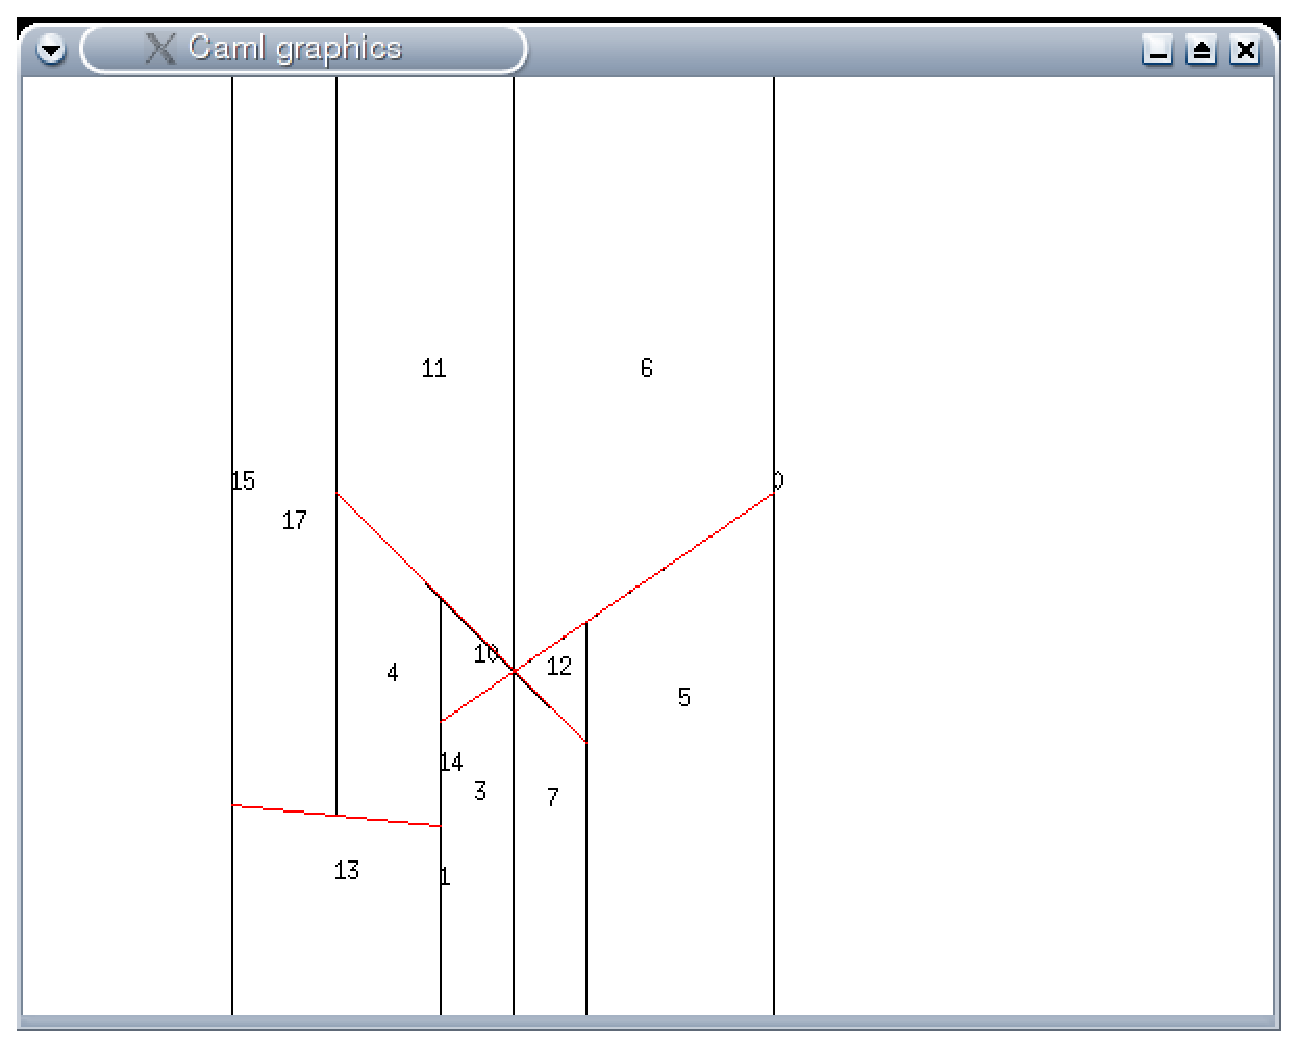
\includegraphics[scale=0.4]{trapdiag1}
  \caption{Trapezoidal map of three line segments}
  \label{fig:trapdiag1}
\end{figure}

\section{Program}

In this section, I will describe each program module summarily. The package
name of the program is known as ``lasvegas-geom'' referring to the
necessarily random nature of the program. Figure 1 depicts the
graphical output of the program for the input of array of line segments:\\
\texttt{
  [| ((100.,100.),(200.,90.));((150.,250.),(270.,130.));\\ ((200.,140.),(360.,250.)) |]}


\subsection{Randomized Incremental Construction}

The construction functor determines types and the basic functions for
construction. As seen, we demand types for the object, regions and a region
set data structure indexed by integers.

Two other important functions are initialization of the region set and a
function to add object to the region set making use of conflict graph. The
implementation is quite straightforward at the moment. It simply adds the
objects in random order from input array using the given functions.

\fvset{fontsize=\small,numbers=left,frame=single, label=module
  Randomizedincr}
\VerbatimInput{randomizedincr.ml}

Since I didn't have a bipartite graph, I used two directed graphs to
implement the conflict graph easily. As a matter of fact, this should grow
to be a bipartite graph implementation because the directed graph calls tend
to be error prone. This code initializes the graph with the required edges
to denote the whole space and each object intersecting with it, which is a
necessary condition.

\fvset{fontsize=\small,numbers=left,frame=single,
  label=module Conflictgraph}
\VerbatimInput{conflictgraph.ml}

\subsection{Line segment intersections}

This module details the input to the functor Randomizedincr.Make which
outputs the complete trapezoidal map construction algorithm.  The code here
deals with maintaining the incremental data structures and calling
appropriate primitive and structural routines.  The bulk of the code here is
concerned with conflict graph and the abstract form of the construction
procedure which may be moved inside the functor. I imagine there could be 2
or 3 more functions to be specified in the input module.

The addition algorithm performs all the steps specified in the paper. It
splits each region that the added object intersects with updating the
conflict graph. Then it merges those regions that can be merged. \footnote{I
  have designed a nice algorithm for this that was not addressed in the
  paper}

Figure \ref{fig:cguse} illustrates how the conflict graph is used when
adding an object from $S-R$ to $F$. Conflict graph keeps track of
intersections between objects in $S-R$ \footnote{Those objects which have
  not yet been added to R} and $F_k$ \footnote{Current set of regions in
  region set}. The figure shows a subgraph of conflict graph. in the graph
shows how an object $oix$ is added from $S-R$ to $R$. The neighbors of $oix$
are regions that $oix$ intersects with. The bold line shows one of the
regions $rix$ that $oix$ intersects with. Naturally $oix$ is a line segment
and $rix$ is a trapezoid here. Once the object $oix$ is added the
trapezoidal diagram and conflict graph must be updated to reflect the
situation. $oix$ is going to split those regions that it intersects with.
The conflict graph will be updated such that objects that intersect with
regions split by $oix$ will be partitioned to new regions. And of course
both $oix$ and the regions it has split will be removed from the graph.  For
instance, we see that $rix$ has edges to $o1, oix, o3, o4$. When $rix$ is
split it is eliminated from the graph leaving its place to two child
trapezoids $c1$ and $c2$ which are added to conflict graph. Since $rix$ will
be gone, its edges must be carried over to $c1$ and $c2$. Each object
intersecting with $rix$, except $oix$ which will be deleted, is subject to
intersection tests to determine the new edges in conflict graph. The
resulting new edges in our hypothetical conflict graph are depicted with
dashed lines.

\begin{figure}[htbp]
  \centering
  \includegraphics[scale=0.6]{cguse}
  \caption{Adding an object to $F_k$ using the conflict graph}
  \label{fig:cguse}
\end{figure}

\subsubsection{Reporting intersections}

Reporting intersections is trivial. In the trapezoid split code, we make
explicit line segment intersection tests while splitting a trapezoid with a
line segment. With a single imperative, the intersections can be accumulated
in an output buffer. I have added a print routine to report the
intersections when detected as an example in \texttt{Trapezoid.split}.

\fvset{fontsize=\small,numbers=left,frame=single,
  label=module Linesegintxn}
\VerbatimInput{linesegintxn.ml}

\subsection{Geometric primitives and structures}

Lineseg module provides for abstraction of line segment and a lot of
geometric primitives required. Of independent interest is a point-line
classification routine and routines for computing intersection of two line
segments, and a line segment and a horizontal/vertical line.

The following module defines a trapezoid record for the trapezoidal map that
is bounded by two line segments from below and above and two vertical lines
from sides. The bounds are potentially open. It also maintains four corner
points. The hardest algorithm in the project is also here, computing how to
split a given trapezoid with a line segment! A trapezoid can be split into
four sub trapezoids, however the computation is not very straightforward.
Also required was a routine to detect the intersection of a trapezoid with a
line segment, that in turn requiring a routine to detect if a point is inside
the trapezoid.

Trapezoidal map is constructed simply from a dynamic array of trapezoids and
an adjacency graph\footnote{Which is not used yet in the code}. The removed
nodes go into a dead list, and are re-used in file organization fashion.  I
am trying to figure out if the adjacency graph is really necessary and if so
how it should be accessed. It has taken a lot of time for me to come up with
this design, as I did not consider DCEL handling these specific trapezoids
in a clean way although it would be the perfect choice if all I needed was a
planar graph.

\subsection{General purpose data structures}

All the data structures used have been designed and implemented from the
very scratch for this project. I have not been able to find high quality
imperative structures that were essential for realizing the running time
bounds.

I have programmed a dynamic array code using open table implementation. This
is a quite useful code and together with a few interfaces it could be
contributed to the Ocaml standard library.

After writing a dynamic array, the adjacency list implementation for graph
data structure becomes a straightforward task. The module interface is quite
fat, but it is worth the bother. Writing module interfaces in separate files
ameliorate code reuse. As can be seen, I have concentrated on the primitive
operations that allow for typical efficient graph algorithms to be written.

I have implemented each adjacency by an ocaml list. The adjacencies are
coupled together using the dynarray type. Since this functional structure
takes care of sharing values it should be as efficient as possible, however
I have not yet seen the performance impact of this. If there is a
performance impact, dynarray can be used instead of the list -- which was
the first implementation of this module. And finally, there is a small
adaptor module for undirected graphs

CLI code and test routines, etc. have been omitted from this section.

\section{Conclusion}

I have reached my goal of being able to program the randomized
incremental construction in a generic way. The program, although short, has
accumulated a lot of programming work. According to SLOCCOUNT by David
Wheeler it has 740 physical source code lines of ML code, totaling to 2.4
months of development time. \footnote{It took three weeks of very hard work
  for me} The geometric primitives and structures are also well
satisfactory. The trapezoidal map construction algorithm is implemented
effectively and it is accompanied with algorithm animation routines which I
have used for graphical debugging.


\end{document}
